% !TEX root = ../thesis.tex

\chapter{Reconstructing Muons in Real Time at the High Luminosity Large Hadron Collider}
\label{chap:TPSappendix}

\section{Introduction}

% Recap of hardware overview in experiment chapter
In chapter~\ref{chap:exp}, we explored the main characteristics of the CMS detector, and in particular, the various subsystems devoted to detecting muons that are produced in collision events.
From its inception, it was recognized that the CMS detector would receive various upgrades over its operational lifetime, and to that end it has already had upgrades installed during its first Long Shutdown (LS1) period~\cite{Battilana:2017mrm,Kreis:2103853}.
At the time of this writing, the LHC is in its Long Shutdown 2 (LS2) phase that began on December 10, 2018, and is projected to resume taking data in 2022~\cite{LHCsched}.

% The existing BMTF
In section~\ref{subsec:trigger} of chapter 3, a brief overview of the CMS trigger system was provided, and the basic architecture of the L1 Trigger was described.
One component of the muon system in the L1 Trigger is the Barrel Muon Track Finder (BMTF), which sorts muon candidates and was commissioned in 2016 for data taking during Run 2~\cite{Ero:2102885}.
The architecture for the BMTF is based on custom processors mounted onto Field Programmable Gate Arrays (FPGAs), with the capability of measuring the transverse momenta of muons in the barrel region.
It was conceived as a replacement for the legacy Drift Tube Track Finder (DTTF), which only received information from the DTs.
The BMTF instead receives superprimitives made from a combination of DT and RPC primitives, which provides better resolution and trigger rates compared to the DTTF.
However, as with other components of the CMS detector, the BMTF is slated to be replaced by newer hardware that offers improvements in performance.

% Appendix overview
In this appendix, we present work towards the implementation of a novel algorithm for reconstructing muon tracks in real time at the LHC.
In section~\ref{sec:CMSUpgrade}, we discuss future upgrades to the CMS detector for Phase 2 that will allow for improvements in muon detection in conjunction with the high luminosity upgrades to the LHC.
Later, in section~\ref{sec:TPS}, we introduce the Tracks Plus Stubs algorithm, which will allow for the reconstruction of muon tracks in real time at the L1 Trigger level.

\section{Future Upgrades to CMS}
\label{sec:CMSUpgrade}

% Phase-2 Upgrades
The High-Luminosity Large Hadron Collider (HL-LHC) is scheduled to come online in 2027, with the Phase-1 period ending in 2024.
During the Long Shutdown 3 (LS3) period in 2025, the CMS detector will undergo major upgrades to its L1 Trigger system~\cite{CERN-LHCC-2020-004}.
Such upgrades are necessary in order to take advantage of the large number of collision events that the HL-LHC will offer, as it will aim for a peak luminosity of $7.5\times10^{34}\unit{cm^{-2}s^{-1}}$.
This will result in up to 200 simultaneous proton-proton collisions per bunch crossing, for which the existing L1 Trigger system is unequipped to handle.
The new L1 Trigger system will have its latency extended from $3.2\unit{\micro s}$ to $12.5\unit{\micro s}$, and it will also have its maximum output bandwidth increased from $100\unit{kHz}$ to $750\unit{kHz}$.
A unique aspect of these upgrades is that the L1 Trigger system will also take information from the inner tracker as input in addition to the muon and calorimeter systems.
This will allow for using the new track finder to provide the initial information about particle transverse momentum \pt, angular position $\phi$, pseudorapidity $\eta$, and charge $q$.
Figure~\ref{fig:P2L1trigger} shows the new architecture of the L1 Trigger that includes the track finder.

\begin{figure}[htbp]
  \centering
  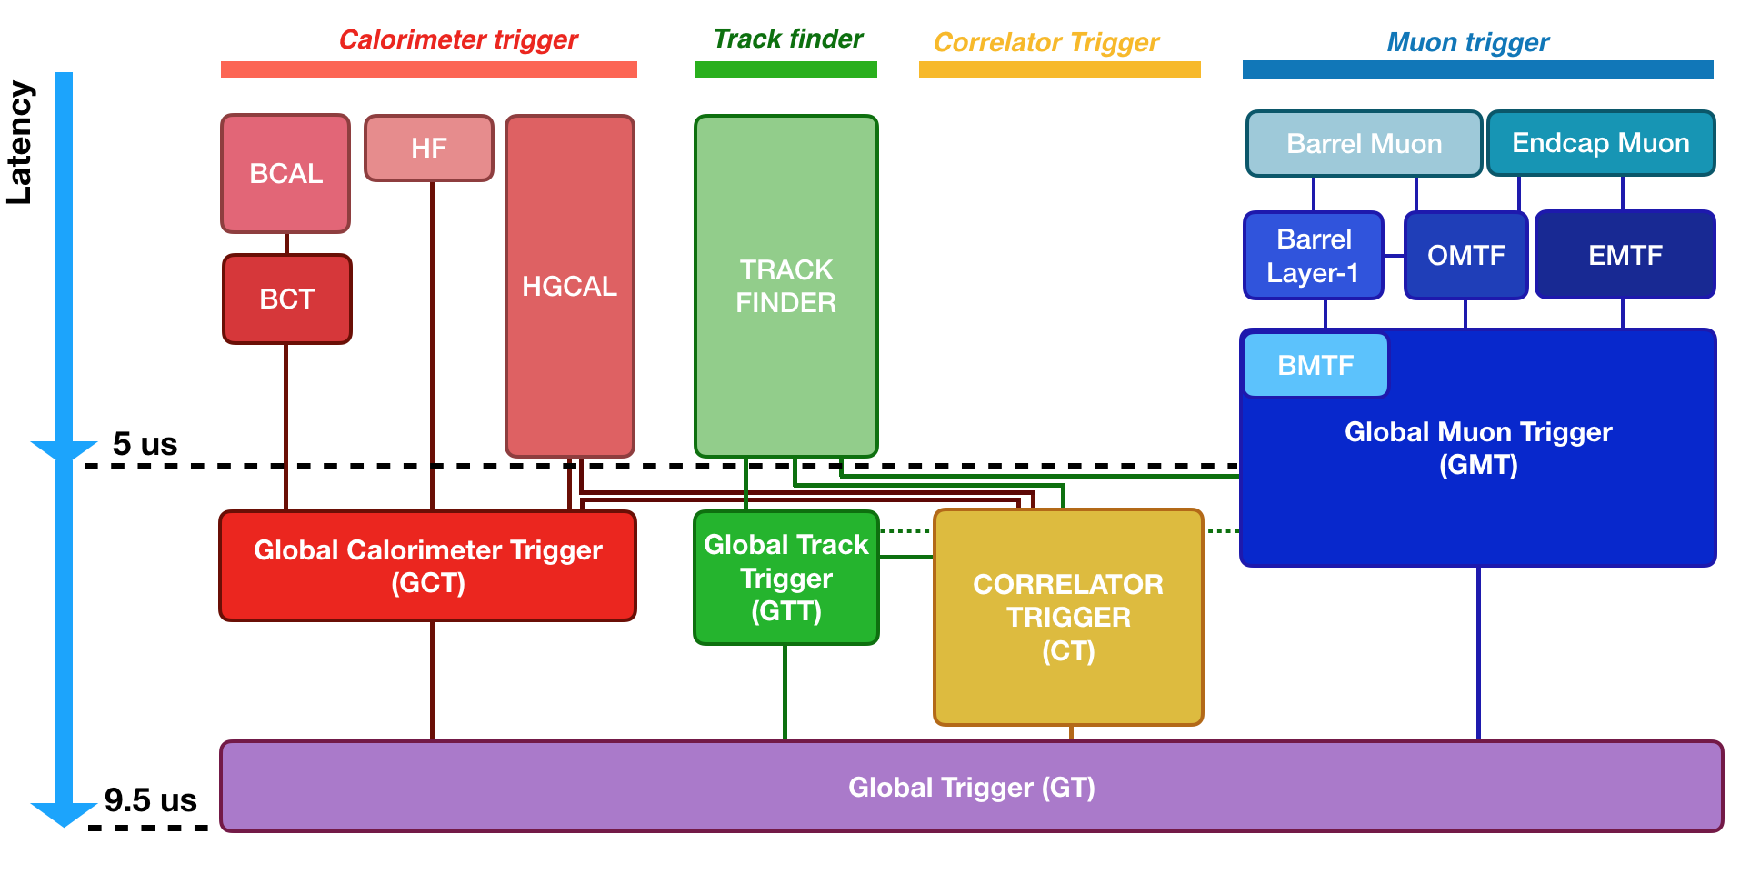
\includegraphics[width=0.85\textwidth]{fig/TPS/P2L1trigger.pdf}
  \caption{
    Architecture of the new L1 Trigger.
    In addition to taking inputs from the calorimeter and muon triggers, the Phase-2 upgrades will include a track finder in the L1 Trigger that takes input from the inner tracker.
  }
  \label{fig:P2L1trigger}
\end{figure}

% The need for new muon trigger algorithms
The prospect of more interactions per bunch crossing is also met with the demand for improvements to muon track reconstruction and resolution.
New algorithms are being developed in order to take advantage of the higher maximum bandwidth and the new track finder in the L1 Trigger.
Some make use of techniques such as Kalman Filters, with an algorithm that can be implemented onto FPGAs for the track trigger~\cite{Amstutz:2194514}, or another for the muon trigger known as the Kalman Barrel Muon Track Finder (KBMTF)~\cite{Bachtis:2648953}.
The work presented in this appendix instead relies on a novel approach to reconstructing muon tracks that uses both the track finder and the muon trigger.

\section{The Tracks Plus Stubs Algorithm}
\label{sec:TPS}

% The tracks plus stubs algorithm
As muons produced in collision events move throughout the detector, they create detection stubs in the DTs, RPCs, and CSCs, which are L1 Trigger primitives that contain information about the angular position $\phi$ and the bending angle $\phi_b$\footnotemark{} in the chamber for which the stub was created.
\footnotetext{The bending angle $\phi_b$ is only measured in the DTs.}
Figure~\ref{fig:CMSslice} shows a slice of the CMS detector in the $r$-$\phi$ plane, with an example of a process in which a muon passes through the DT chambers~\cite{Barney:2120661}.
The Tracks Plus Stubs (TPS) algorithm combines the information from the track trigger and the detection stubs in the chambers to create a candidate track that will later be reconstructed as a muon in the detector.
By using the initial information from the track trigger, the algorithm propagates the initial muon track to the outer layers of the detector.
The propagated values for the angular variables $\phi$ and $\phi_b$ are then compared to those as recorded by the stub measurements.
From this, the algorithm can construct a candidate muon track, which is a combined object consisting of a track from the track trigger, and a collection of stubs associated to the track.

\begin{figure}[htbp]
  \centering
  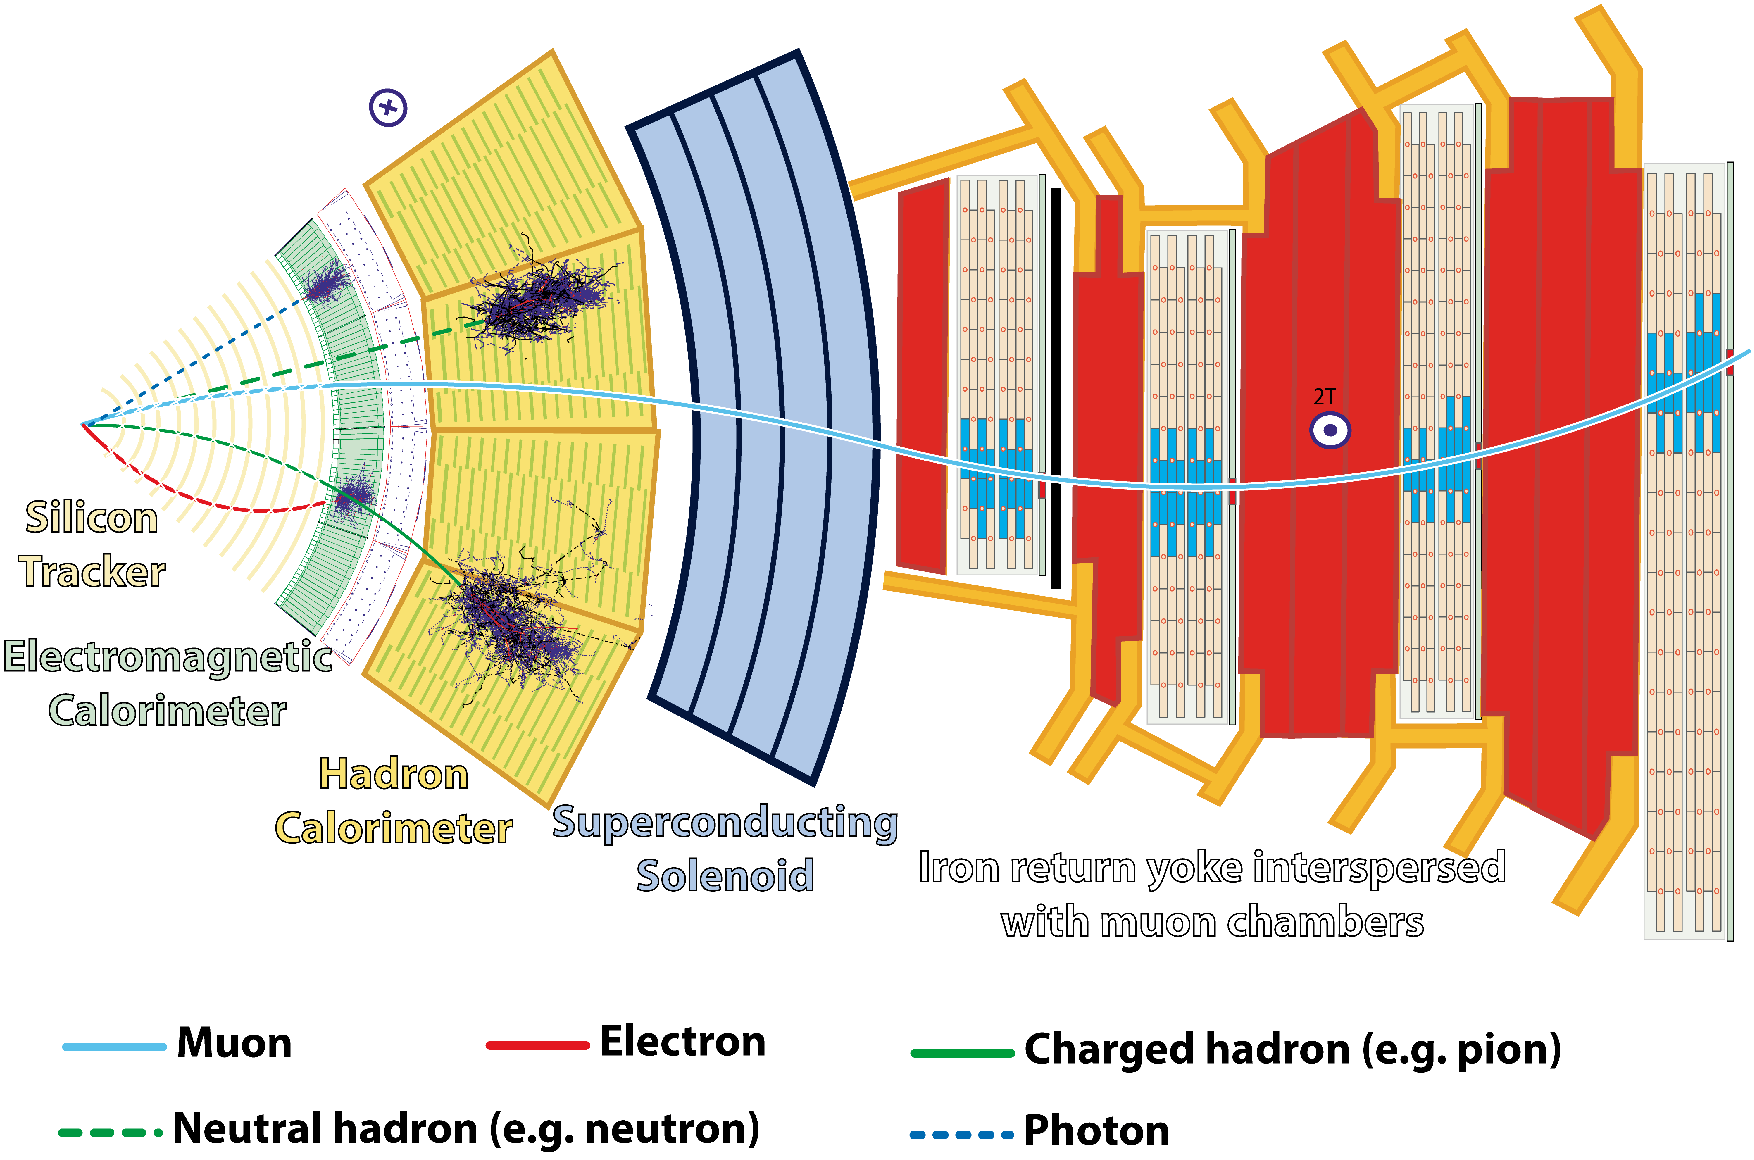
\includegraphics[width=0.85\textwidth]{fig/TPS/CMSslice_whiteBackground.pdf}
  \caption{
    Slice of the CMS detector for a process in which a muon is produced.
    As the muon passes through the silicon tracker and the muon chambers, the electronics obtain measurements of the muon's transverse momentum \pt, angular position $\phi$, pseudorapidity $\eta$, and charge $q$.
    Such information is used by the L1 Trigger to decide whether or not to save an event for analysis.
  }
  \label{fig:CMSslice}
\end{figure}

\subsection{Muon Track Propagation}
\label{subsec:prop}

% Transverse momentum in a uniform magnetic field
One of the defining characteristics of the CMS detector is the $3.8\unit{T}$ solenoidal magnetic field that is aligned with the beam axis.
In a uniform magnetic field $B$, a charged particle of charge $q$ with momentum transverse to the magnetic field \pt will experience an induced centripetal force due to the Lorentz force that the magnetic field exerts on the charge.
This in turn defines a radius of orbit $R$ for the charge, which is related to the transverse momentum \pt by the relation $\pt=qBR$. It is typical in particle physics to convert the units of the elementary charge so that in terms of $B$ and $R$, we have
\begin{equation}\label{eq:pt}
  \pt=0.3BR\unit{GeV/\clight}.
\end{equation}

% Parabolic approximation of track
However, it is too computationally expensive to use the exact formula for a circular arc in the L1 Trigger hardware in order to model the trajectory that a charged particle takes through the detector.
Moreover, the transverse momenta for muons that result in a typical collision event of interest are such that a parabolic approximation is accurate enough to describe the track of the particle.

% Derivation of position and bending angles
Assuming that the track starts in the center of the beamline as in figure~\ref{fig:arc}, we may approximate the circular arc that the charged particle follows through the detector by
\begin{equation}\label{eq:para}
  y(x)=\frac{x^2}{2R}+bx,
\end{equation}
where $R$ is the radius of curvature as in Eq.~\ref{eq:pt}, and $b$ is a constant to be determined.
First, observe that at the origin, the tangent of the initial angle $\phi_0$ corresponds to the first derivative of~\ref{eq:para} evaluated at $x=0$. Therefore,
\begin{equation}
  \eval{\dv{y}{x}}_{x=0}=\tan\phi_0=b,
\end{equation}
and hence
\begin{equation}
  y(x)=\frac{x^2}{2R}+x\tan\phi_0.
\end{equation}
At the position of the charge $q$, we also have that the tangent of the position angle $\phi$ is given by
\begin{equation}
  \tan\phi=\frac{y(x_\mathrm{stub})}{x_\mathrm{stub}}=\frac{x_\mathrm{stub}}{2R}+\tan\phi_0,
\end{equation}
which we may rearrange to obtain
\begin{equation}
  \tan\phi-\tan\phi_0=\frac{x_\mathrm{stub}}{2R}.
\end{equation}
Since the \pt of a muon that passes through the threshold of the detector is high enough such that the radius $R$ is large, $\Delta\phi\equiv\phi-\phi_0$ is small, and hence we may make the approximation that $\tan\phi-\tan\phi_0\approx\phi-\phi_0$.
Thus,
\begin{equation}\label{eq:phi}
  \phi=\frac{x_\mathrm{stub}}{2R}+\phi_0=ck+\phi_0,
\end{equation}
where we have used the fact that $k=1/R$ and $c$ is a constant to be determined based on the position of the stub.
Furthermore, in figure~\ref{fig:arc}, we can see that due to the symmetry of the circular arc traced by the track of the particle, the bending angle $\phi_b$ must be equal to the change in the position angle $\Delta\phi$, and hence we immediately obtain
\begin{equation}\label{eq:phib}
  \phi_b=ck.
\end{equation}

\begin{figure}[htbp]
  \centering
  % !TEX root = ../../thesis.tex
\begin{tikzpicture}
  % Axes
  \draw[->] (0,0) -- (2,0) node[below] {$x$};
  \draw[->] (0,0) -- (0,2) node[left] {$y$};

  % Arc
  \coordinate (q) at ($(120:5)+(15:5)$);
  \draw[fill=black] (120:5) circle (1pt);
  \draw[red] (0,0) arc (-60:15:5);
  \draw[->,thick,red] (q) -- ($(q)+(105:1)$) node[left,red] {$\vb{p}_\mathrm{T}$};
  \draw[red,dashed] (0,0) -- (30:2);

  % Lines
  \draw[dashed] (0,0) -- (120:5) node[pos=0.5,left] {$R$};
  \draw[dashed] (120:5) -- (q) node[pos=0.5,above] {$R$};
  \draw[dashed] (67.5:3.044) -- ($(120:5)+(-22.5:5)$) node[pos=0.5,above] {$s$};

  % Angles
  \draw[red] (0.75,0) arc (0:30:0.75) node[pos=0.75,right,red] {$\phi_0$};
  \draw[cyan] (0.5,0) arc (0:67.5:0.5) node[pos=0.8,above right,cyan] {$\phi$};
  \draw (30:1.25) arc (30:67.5:1.25) node[pos=0.8,above right] {$\Delta\phi$};
  \draw[cyan,dashed] (q) -- ($(q)+(67.5:1)$);
  \draw[red] ($(q)+(67.5:0.5)$) arc (67.5:105:0.5) node[pos=0.35,above,red] {$\phi_b$};

  % Charge
  \draw[cyan] (0,0) -- (q) node[pos=0.5,left,cyan] {$L$}; % 6.088
  \draw[fill=cyan] (q) circle (2.5pt) node [right,cyan] {$q$};
  \draw ($(q)+(1.25,-0.5)$) node {$(x_\mathrm{stub},y_\mathrm{stub})$};
\end{tikzpicture}

  \caption{Illustration of the circular trajectory taken by a particle with charge $q$ positioned at $(x_\mathrm{stub},y_\mathrm{stub})$ in a uniform magnetic field. The track starts at the origin with an initial angle $\phi_0$ tangent to the track of the particle, and ends with a final angle of $\phi$ for a total change in angle $\Delta\phi\equiv\phi-\phi_0$. The charged particle covers a radial distance $L$ with respect to the origin of the track, and the perpendicular distance between the mid-point of the track and the radial line $L$ is denoted by the sagitta $s$. The vector corresponding to the \pt of the charge is labeled, with the bending angle $\phi_b$ drawn with respect to the radial line $L$.}
  \label{fig:arc}
\end{figure}

% Geometric significance of propagation coefficients
With equations~\ref{eq:phi} and~\ref{eq:phib} in hand, we may now propagate the tracks based on the initial information about the curvature $k$ and angle $\phi_0$.
The CMS detector consists of multiple layers of detection chambers, and each chamber requires its own propagation constant $c$.
The relevant variables to consider for $c$ based on the geometry of the detector are the pseudorapidity of the track $\eta$ and the station depth $d$.
Thus, the propagation constants $C(\eta,d)$ are functions of these two variables.
Rather than obtaining these constants analytically, they are obtained by using simulation data. % Elaborate on the simulation samples used later

% Obtaining propagation coefficients
To do this, we divide the detector into separate $\eta$ regions and depths, as seen in figure~\ref{fig:barrelEta}, and treat each section as a separate detector with its own propagation constant $c(\eta,d)$.
We then look at two-dimensional histograms of $\Delta\phi$ and $\phi_b$ from simulated detection stubs as functions of $k$ for each section of the detector based on simulated detection stubs.
An example of this can be seen in figure~\ref{fig:deltaPhiHist}.
For every bin in curvature $k$, the distribution of $\Delta\phi$ or $\phi_b$ is roughly Gaussian, and hence we fit Gaussians to the vertical slices of these histograms.
We then consider the mean of these Gaussians and make linear fits for $\Delta\phi$ and $\phi_b$ in accordance with equations~\ref{eq:phi} and~\ref{eq:phib}.
These then define the propagation constants $c(\eta,d)$ for each detector, thereby allowing us to predict where a muon produced at the beamline during a collision event will end up in the detection chambers.

\begin{figure}[htbp]
  \centering
  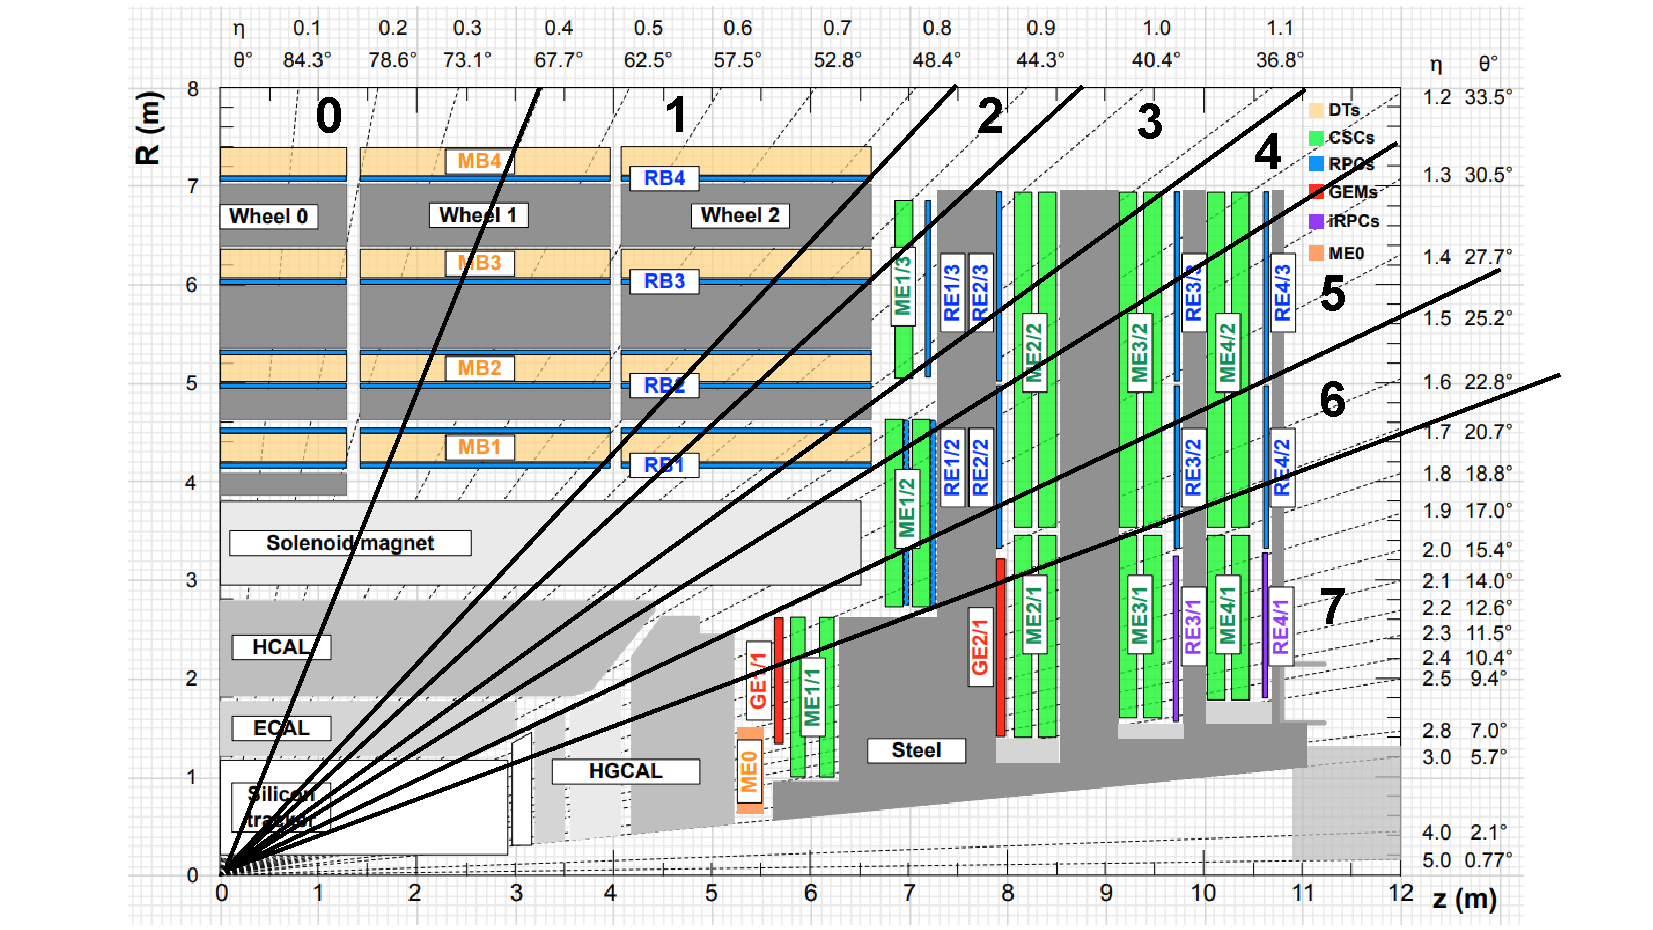
\includegraphics[width=0.85\textwidth]{fig/TPS/barrelEta.pdf}
  \caption{Cross section of the CMS detector in the $r$-$z$ plane illustrating how the detector is separated into different $\eta$ regions. Each $\eta$ region and depth is treated as a separate detector for the TPS algorithm.}
  \label{fig:barrelEta}
\end{figure}

\begin{figure}[htbp] % Need to update figure
  \centering
  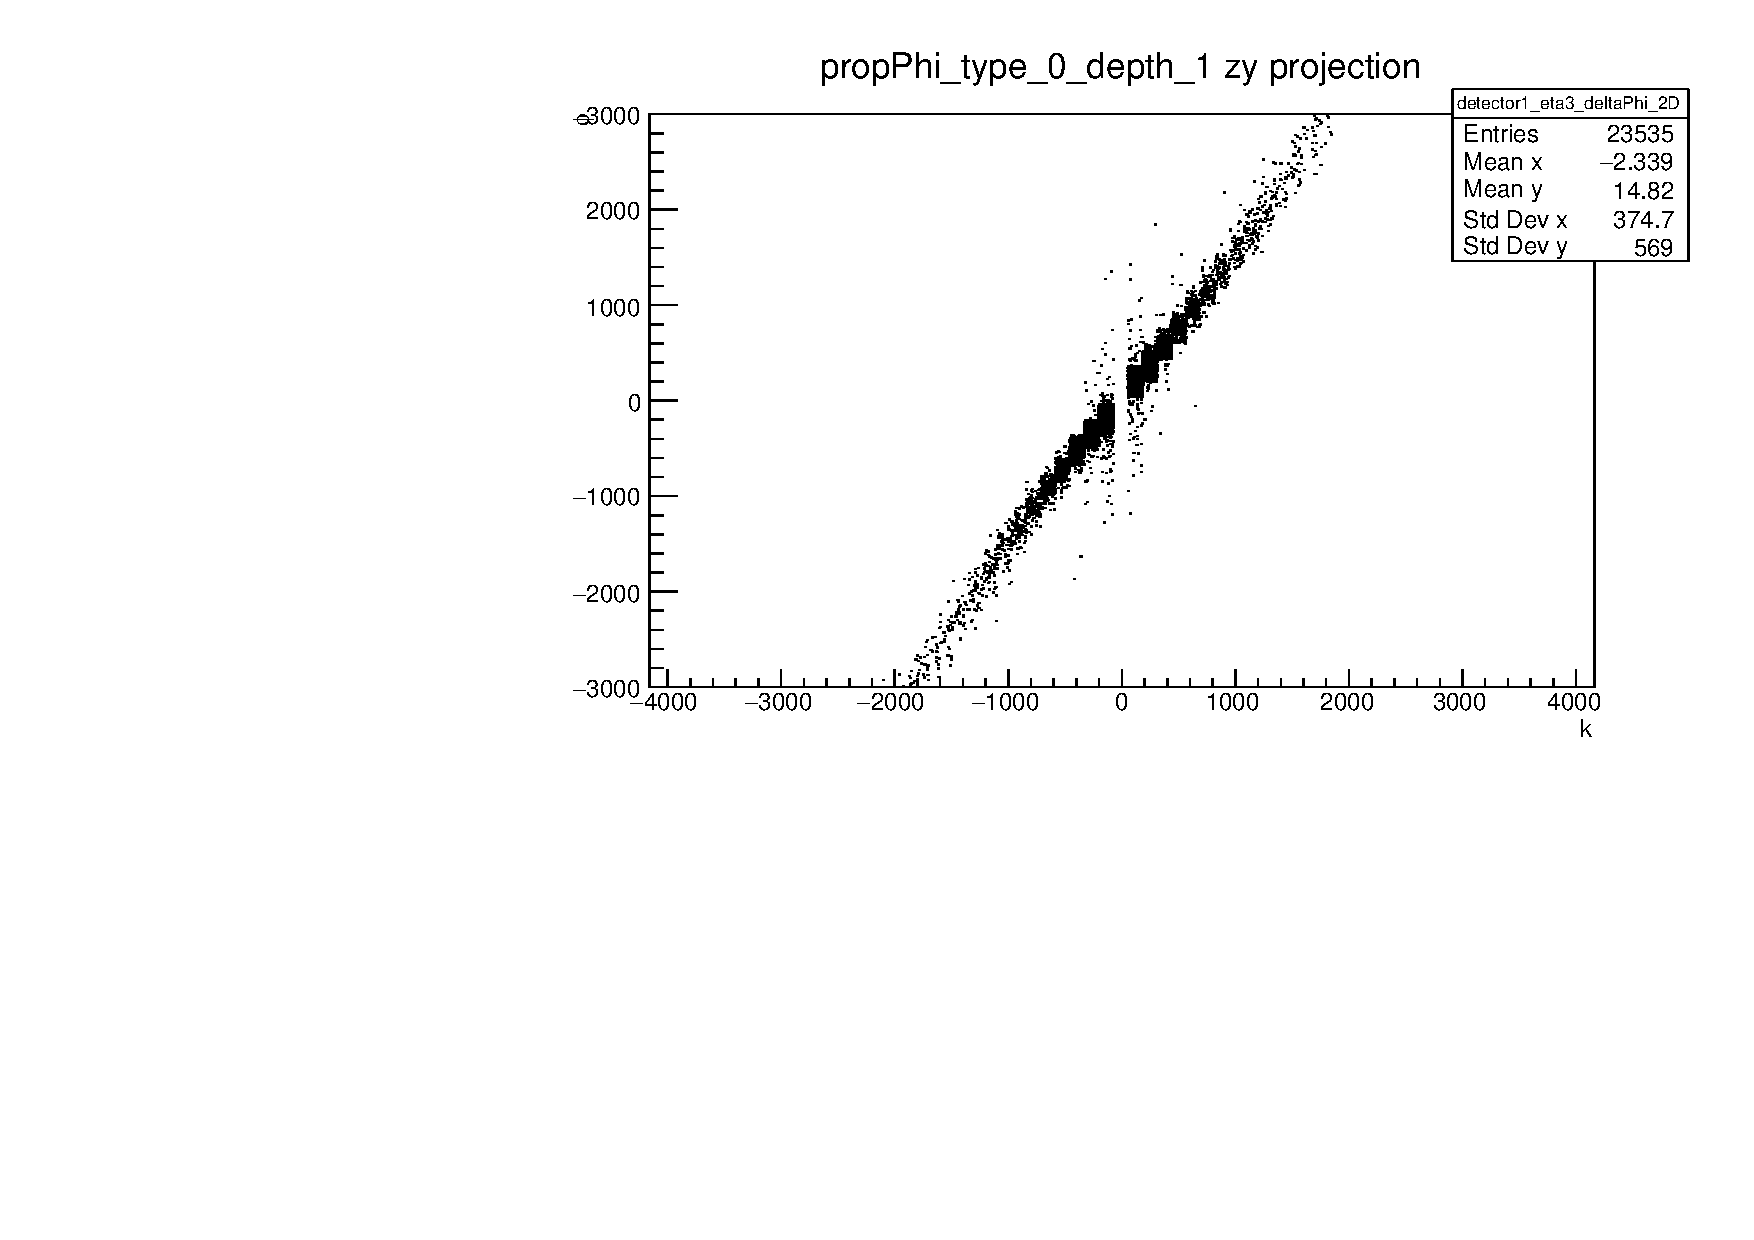
\includegraphics[width=0.48\textwidth]{fig/TPS/deltaPhi_2D.pdf}
  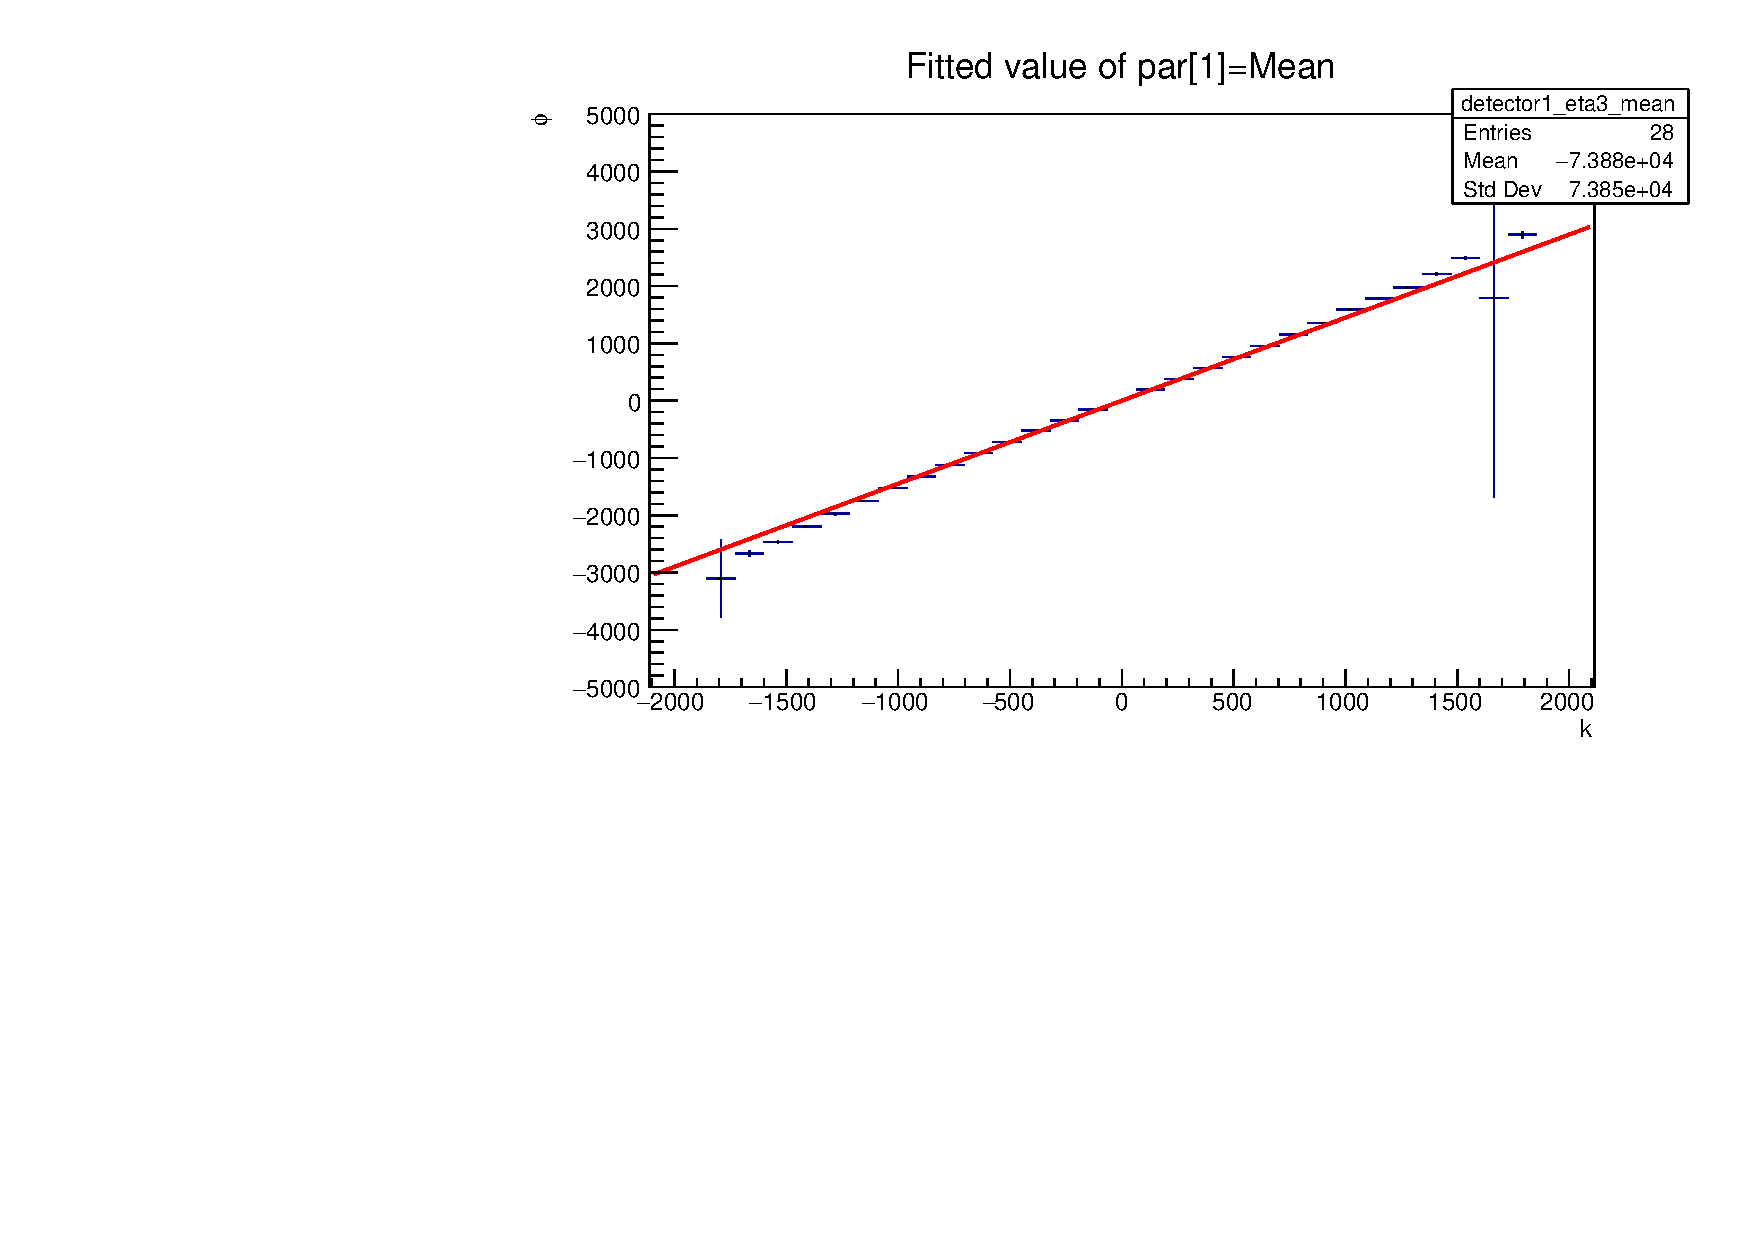
\includegraphics[width=0.48\textwidth]{fig/TPS/deltaPhi_mean.pdf}
  \caption{Two-dimensional distribution of $\Delta\phi$ from simulated detection stubs as a function of curvature $k$ (left), and linear fit for the mean values of Gaussians fitted to the vertical slices of the two-dimensional histogram (right). Propagation constants $c(\eta,d)$ for $\Delta\phi$ and $\phi_b$ for each section of the detector are obtained through these linear fits, in accordance with equations~\ref{eq:phi} and~\ref{eq:phib}.}
  \label{fig:deltaPhiHist}
\end{figure}

\subsection{Pull Distributions and Stub Matching}
\label{subsec:pulls}

% Position resolution
Once the propagation constants are obtained, the information for a candidate muon obtained from the track trigger can be used to predict where the muon detection stubs will be found in the detector based on the initial information about the curvature of the track $k$ and the initial angle $\phi_0$.
One of the main considerations in matching a track to detection stubs is the position resolution for the stub measurements.
The standard deviation of the Gaussian fits for $\Delta\phi$ and $\phi_b$ as described in the previous subsection corresponds to the position resolution of the measurements, and has a quadratic form
\begin{equation}
  \sigma=\sqrt{\alpha k^2+\beta},
\end{equation}
where $\alpha$ is a multiple scattering term that dominates for high curvature tracks (i.e., low $p_\mathrm{T}$ tracks), and $\beta$ is a constant term corresponding to the position uncertainty of the detector \cite{PhysRevD.98.030001}.

% Linear approximation for resolution
However, this form for $\sigma$, as with the analytic forms for the propagated $\phi$ and $\phi_b$ values, is too computationally expensive to implement into the hardware.
Instead, we approximate the position resolution using
\begin{equation}\label{eq:posRes}
  \sigma\approx a|k|+b,
\end{equation}
where $a$ and $b$ are constants analogous to $\alpha$ and $\beta$.
Figure~\ref{fig:deltaPhiRes} shows an example of the position resolution from one of the Gaussian fits for $\Delta\phi$ and the fit obtained for equation~\ref{eq:posRes}.
As with the propagation coefficients $c(\eta,d)$, the position resolution constants $a(\eta,d)$ and $b(\eta,d)$ are also specific to each detector based on the $\eta$ region and depth.

\begin{figure}[htbp] % Need to update figure
  \centering
  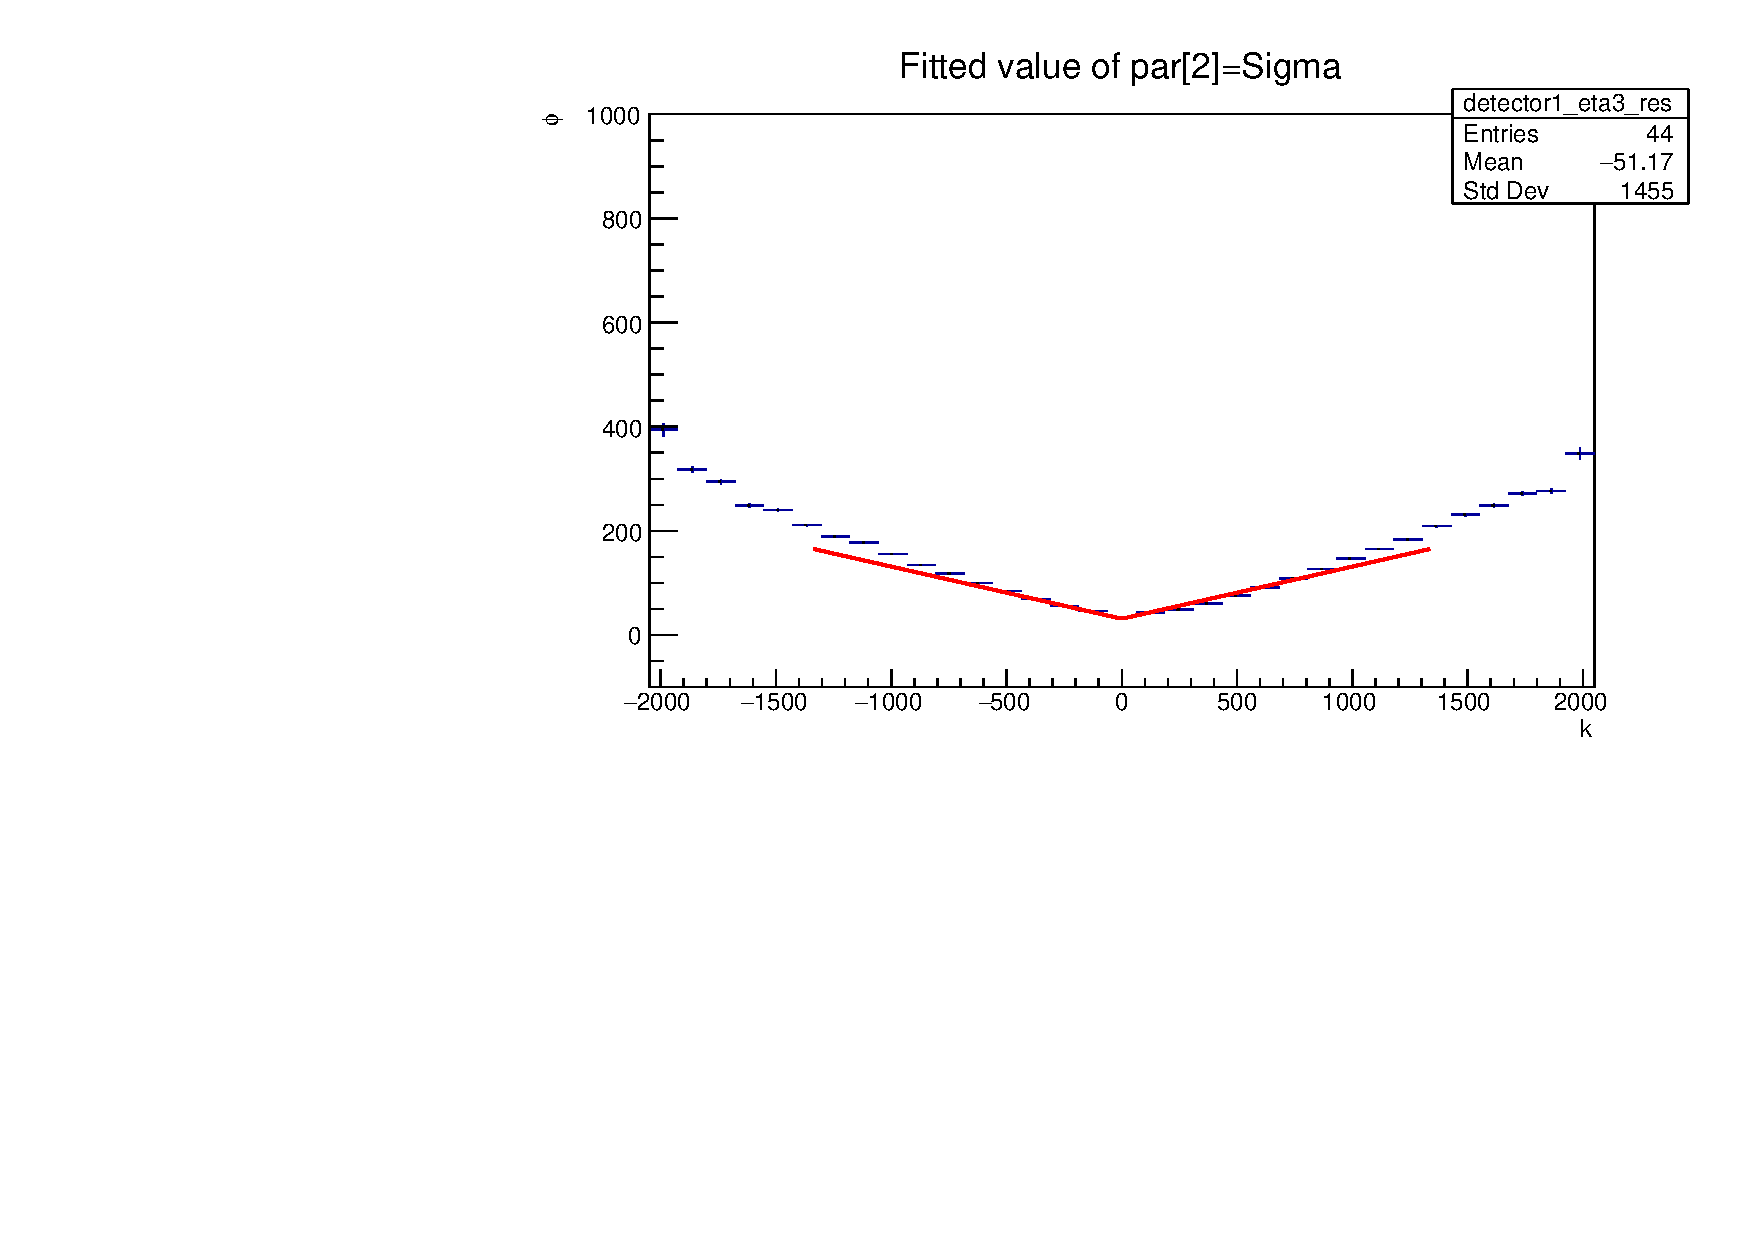
\includegraphics[width=0.48\textwidth]{fig/TPS/deltaPhi_res.pdf}
  \caption{Plot of the resolution for the stub measurements based on the Gaussian fits obtained from the two-dimensional distributions of $\Delta\phi$. The resolution is fitted using the linear approximation of equation~\ref{eq:posRes}.}
  \label{fig:deltaPhiRes}
\end{figure}

% Selecting stubs based on pull values
With the means to propagate the tracks from the track trigger and determine the resolution of the stub measurements, we may now proceed with determining whether or not a stub is suitable for being matched with a candidate muon.
To do this, we consider the pull distributions for each stub with respect to a track.
For each track, we check the pull values of every stub that may get matched with the track, which are given by
\begin{equation}\label{eq:pull}
  P_\phi=\frac{\phi_\mathrm{prop}-\phi_\mathrm{stub}}{\sigma}=\frac{\phi_\mathrm{prop}-\phi_\mathrm{stub}}{a|k|+b}.
\end{equation}
The distributions made by sampling these pull values from simulation are Gaussian distributed, and an example may be seen in figure~\ref{fig:deltaPhiPull}.
We then match stubs to tracks by considering the absolute value of the pulls for each stub.
If $|P_\phi|$ for a stub is below a certain threshold for a track, then the stub will be matched to the track.
Stubs that exceed the threshold for $|P_\phi|$ will instead be discarded.

\begin{figure}[htbp] % Need to update figure
  \centering
  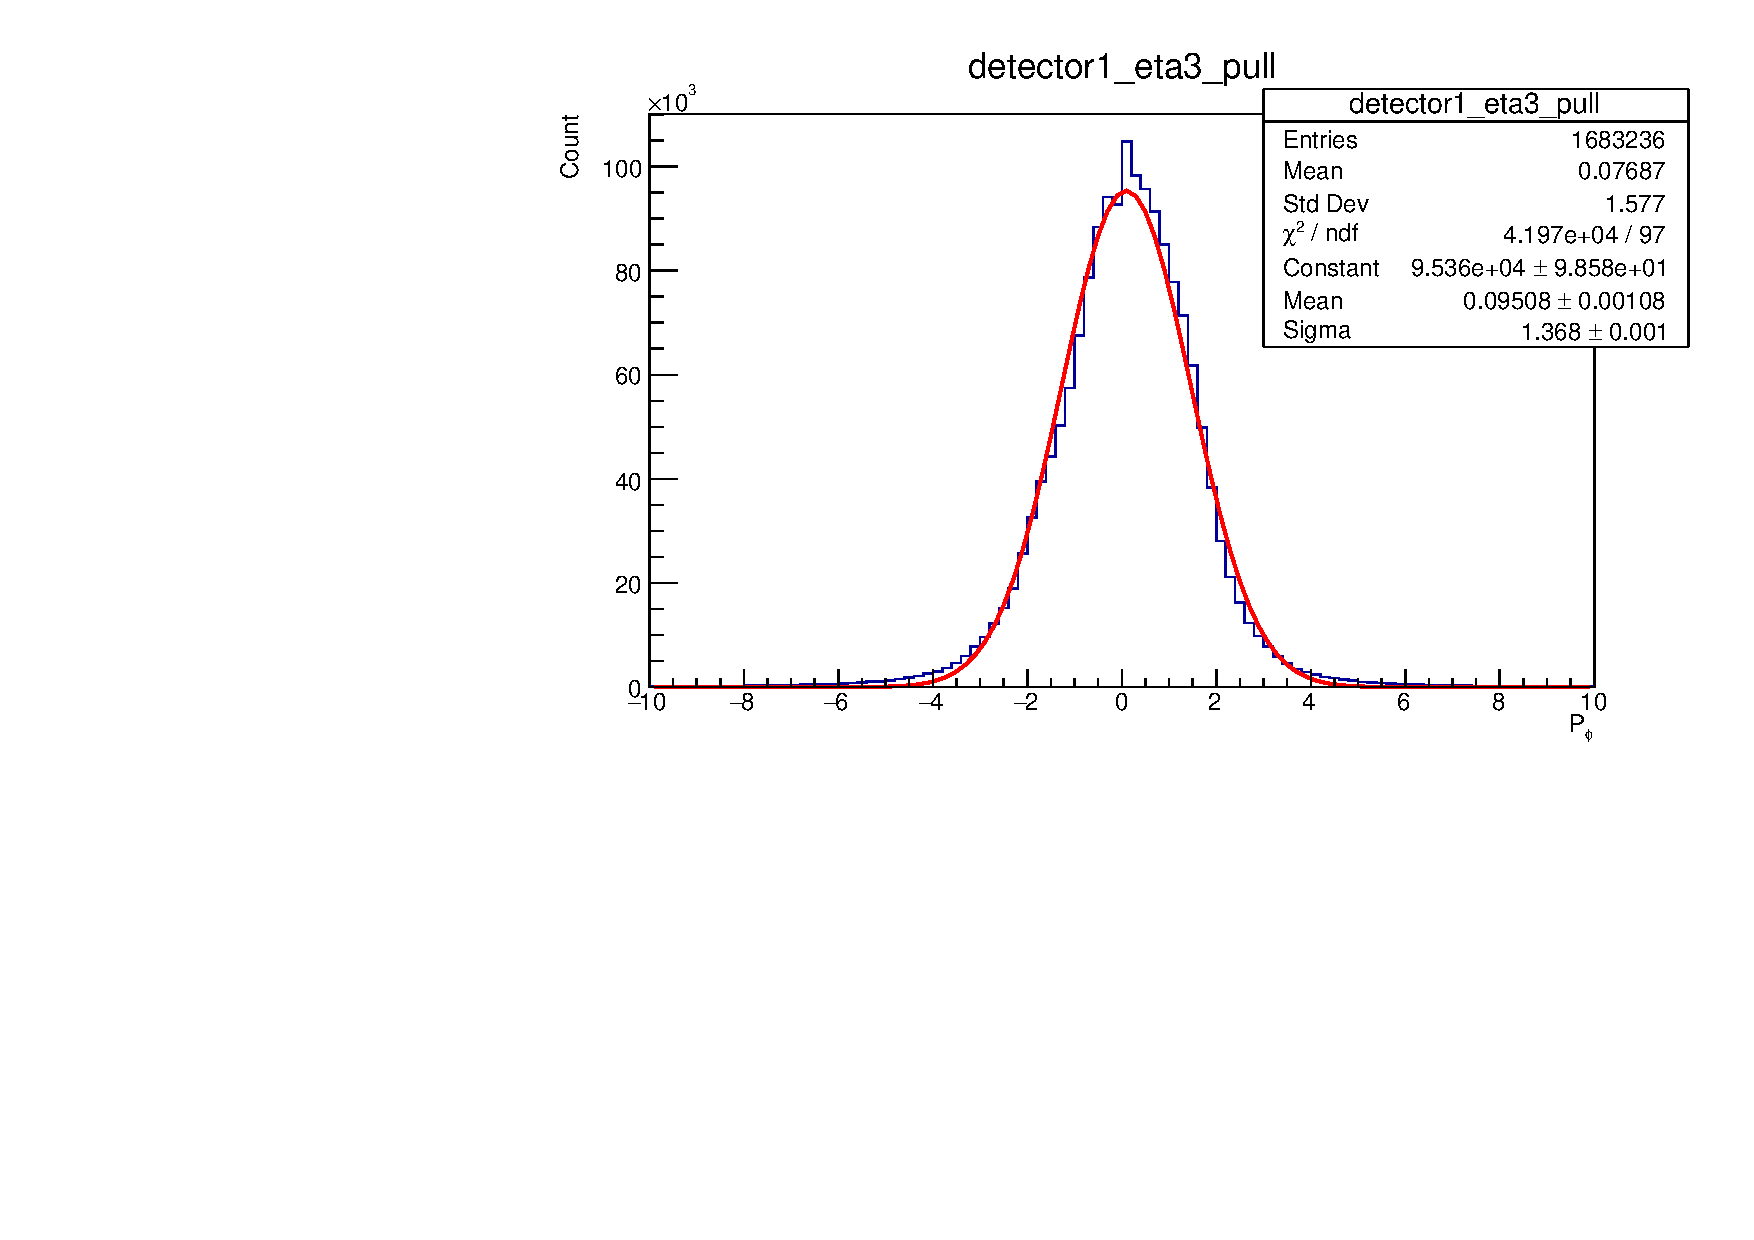
\includegraphics[width=0.48\textwidth]{fig/TPS/deltaPhi_pull.pdf}
  \caption{Example of a pull distribution for a single section of the detector based on the depth and $\eta$ region. The histogram is made by sampling the pull values of all tracks in simulation based on equation~\ref{eq:pull}. By construction, the pull distribution is a Gaussian with a mean of 0 and a standard deviation of 1.}
  \label{fig:deltaPhiPull}
\end{figure}

% Put figures and explanation for how the pull distributions are highly correlated with signal and uncorrelated with background

\subsection{Track Cleaning and Isolation}
\label{subsec:cleaning}

% The need for stub cleaning
One issue that arises in the course of matching stubs to tracks is the possibility of having more than one detection stub shared between tracks.
As a stub can only come from a single muon track, the algorithm requires a process by which tracks are discarded if they share one or more stubs.
To deal with this, the TPS algorithm cleans tracks by checking if there are stubs shared between tracks after all the candidate tracks are obtained.

% Stub cleaning process
There are two cases that are considered during the cleaning process.
The first is case 1 in figure~\ref{fig:clean}, in which two or more tracks share one or more detection stubs. In this case, the track with the most detection stubs is retained and all others are discarded.
For case 2, if two tracks have the same number of stubs, we instead consider the difference in the propagated values of $\phi$ versus the values as measured by the detection stubs.
We evaluate the sum of the difference in these values by evaluating
\begin{equation}\label{eq:phiDev}
  \Delta\phi_{\mathrm{prop,sum}}=\sum_i|\phi_{\mathrm{prop},i}-\phi_{\mathrm{stub},i}|,
\end{equation}
where $i$ denotes the depth in the detector, for each candidate track.
The track with the smallest sum $\Delta\phi_{\mathrm{prop,sum}}$ of the deviation in $\phi$ between the propagated and stub measured value is retained, while all others are discarded.

\begin{figure}[htbp]
  \centering
  % !TEX root = ../../thesis.tex
\begin{tikzpicture}
  % Tracks Case 1
  \draw[red] (0,0) arc (-80:-20:3);
  \draw[orange] (0,0) arc (-100:-10:3.5);

  % Tracks Case 2
  \draw[red] (8,0) arc (-80:-10:3.25);
  \draw[orange] (8,0) arc (-100:-10:3.5);

  % Stubs Case 1
  \draw[fill=black] (10:1) circle (1pt);
  \draw[fill=black] (16:2) circle (1pt);
  \draw[fill=black] (22:3) circle (1pt);
  \draw[fill=black] (28:4) circle (1pt);

  % Stubs case 2
  \draw[fill=black] ($(8,0)+(7:1)$) circle (1pt);
  \draw[fill=black] ($(8,0)+(12:2)$) circle (1pt);
  \draw[fill=black] ($(8,0)+(20:3)$) circle (1pt);
  \draw[fill=black] ($(8,0)+(27:4)$) circle (1pt);

  % Labels Case 1
  \draw (2,3.25) node {Case 1:};

  \draw[red,->] (0,1) -- (10:1);
  \draw[red,->] (0,1) -- (16:2);
  \draw (0,1) node[red,fill=white,inner sep=2pt] {Track 1 Stubs};

  \draw[orange,->] (4,0) -- (10:1);
  \draw[orange,->] (4,0) -- (16:2);
  \draw[orange,->] (4,0) -- (22:3);
  \draw[orange,->] (4,0) -- (28:4);
  \draw (4,0) node[orange,fill=white,inner sep=2pt] {Track 2 Stubs};

  % Labels Case 2
  \draw (10,3.25) node {Case 2:};

  \draw[red,->] (8,1) -- ($(8,0)+(7:1)$);
  \draw[red,->] (8,1) -- ($(8,0)+(12:2)$);
  \draw[red,->] (8,1) -- ($(8,0)+(20:3)$);
  \draw[red,->] (8,1) -- ($(8,0)+(27:4)$);
  \draw (8,1) node[red,fill=white,inner sep=2pt] {Track 1 Stubs};

  \draw[orange,->] (12,0) -- ($(8,0)+(7:1)$);
  \draw[orange,->] (12,0) -- ($(8,0)+(12:2)$);
  \draw[orange,->] (12,0) -- ($(8,0)+(20:3)$);
  \draw[orange,->] (12,0) -- ($(8,0)+(27:4)$);
  \draw (12,0) node[orange,fill=white,inner sep=2pt] {Track 2 Stubs};
\end{tikzpicture}

  \caption{Illustration of the two different cases that are considered when cleaning candidate tracks that share detection stubs. In case 1 there are two tracks that share stubs but one track has more stubs than the other. In case 2, the tracks share the same number of stubs, but one track has a smaller sum of the deviation in the propagated $\phi$ values as given in equation~\ref{eq:phiDev}.}
  \label{fig:clean}
\end{figure}

% Track isolation process
The TPS algorithm also allows for track isolation when considering muon candidates in order to reduce heavy flavor contributions from QCD processes, which allows for reducing background.
For each candidate track, the algorithm checks to see if there are any additional tracks whose origin is within $dz<0.2\unit{cm}$ along the beamline of the candidate track's origin, and if these tracks are within a cone of radius $\Delta R$ centered around the candidate track, as seen in figure~\ref{fig:isol}.
The algorithm then evaluates the sum of the individual transverse momenta $p_{\mathrm{T},i}$ given by
\begin{equation}\label{eq:ptCone}
  p_\mathrm{T,cone}=\sum_{i\in\mathrm{cone}}p_{\mathrm{T},i},
\end{equation}
where we exclude the candidate track for which the cone is centered upon.
If $p_\mathrm{T,cone}$ exceeds the threshold set for the algorithm, then the candidate track being evaluated is discarded.

\begin{figure}[htbp]
  \centering
  % !TEX root = ../../thesis.tex

\begin{tikzpicture}
  % Axis
  \draw[->] (0,0) -- (8,0) node[right] {$z$};

  % Tracks
  \draw[fill=black] (1,0) circle (1pt);
  \draw[fill=black] (3.5,0) circle (1pt);
  \draw[fill=black] (4,0) circle (1pt);
  \draw[fill=black] (7,0) circle (1pt);
  \draw[->,thick] (1,0) -- ($(1,0)+(105:2)$);
  \draw[->,thick] (3.5,0) -- ($(3.5,0)+(75:3)$);
  \draw[->,thick] (4,0) -- ($(4,0)+(110:3.5)$) node[above] {TPS $\mu$};
  \draw[->,thick] (7,0) -- ($(7,0)+(80:2.5)$);

  % Cone
  \draw[rotate around={20:(4,0)},dotted] (4,2) ellipse (1.3 and 0.6);
  \draw[rotate around={20:(4,0)},dotted] (4,0) -- ($(4,0)+(55.725:2.25)$);
  \draw[rotate around={20:(4,0)},dotted] (4,0) -- ($(4,0)+(124.275:2.25)$);

  % Labels
  \draw[|-|] (3.5,-0.25) -- (4,-0.25) node[below] {$|dz|<0.2$ cm};
  \draw (5.5,2.75) node {$\Delta R=0.5$};
\end{tikzpicture}

  \caption{Illustration of the track isolation process used by the algorithm. A cone is defined about the origin of the candidate track TPS $\mu$ and the algorithm checks if there are any adjacent tracks whose origin is within $dz$ of the TPS $\mu$ origin, and if the track is within a cone of radius $\Delta R$ centered about TPS $\mu$. Tracks for which $p_\mathrm{T,cone}$ as defined by equation~\ref{eq:ptCone} exceeds the threshold set for the algorithm are discarded.}
  \label{fig:isol}
\end{figure}

\subsection{Trigger Efficiencies and Rates}
\label{subsec:effRates}

% Trigger efficiency definition
To assess the effectiveness in the algorithm, efficiency studies were performed to see how well the algorithm matches stubs to real muon tracks in simulation.
For a given event, the efficiency is defined by
\begin{equation}\label{eq:eff}
  \epsilon=\frac{N_\mathrm{TPS}}{N_\mathrm{gen}},
\end{equation}
where $N_\mathrm{TPS}$ is the number of TPS tracks obtained by the algorithm, and $N_\mathrm{gen}$ is the number of real muons generated in the simulation event.
Figure~\ref{fig:eff} shows the results obtained when evaluating the efficiency for all events in a simulation sample of muons passing through the detector as a function of muon $\eta$ (left) and \pt (right).
The performance of the TPS algorithm is compared to the existing BMTF, K-BMTF, and Technical Proposal (TP) algorithms.
For these efficiency studies, we required that a TPS track has at least two stubs.
A notable feature of the TPS algorithm is its performance in the gap region of $|\eta|\in[0.15,0.35]$ between wheels 1 and $-1$.
While other algorithms suffer significant losses in efficiency in the gap region, the TPS algorithm performs especially well by comparison on this region.

\begin{figure}[htbp] % Need to update figure
  \centering
  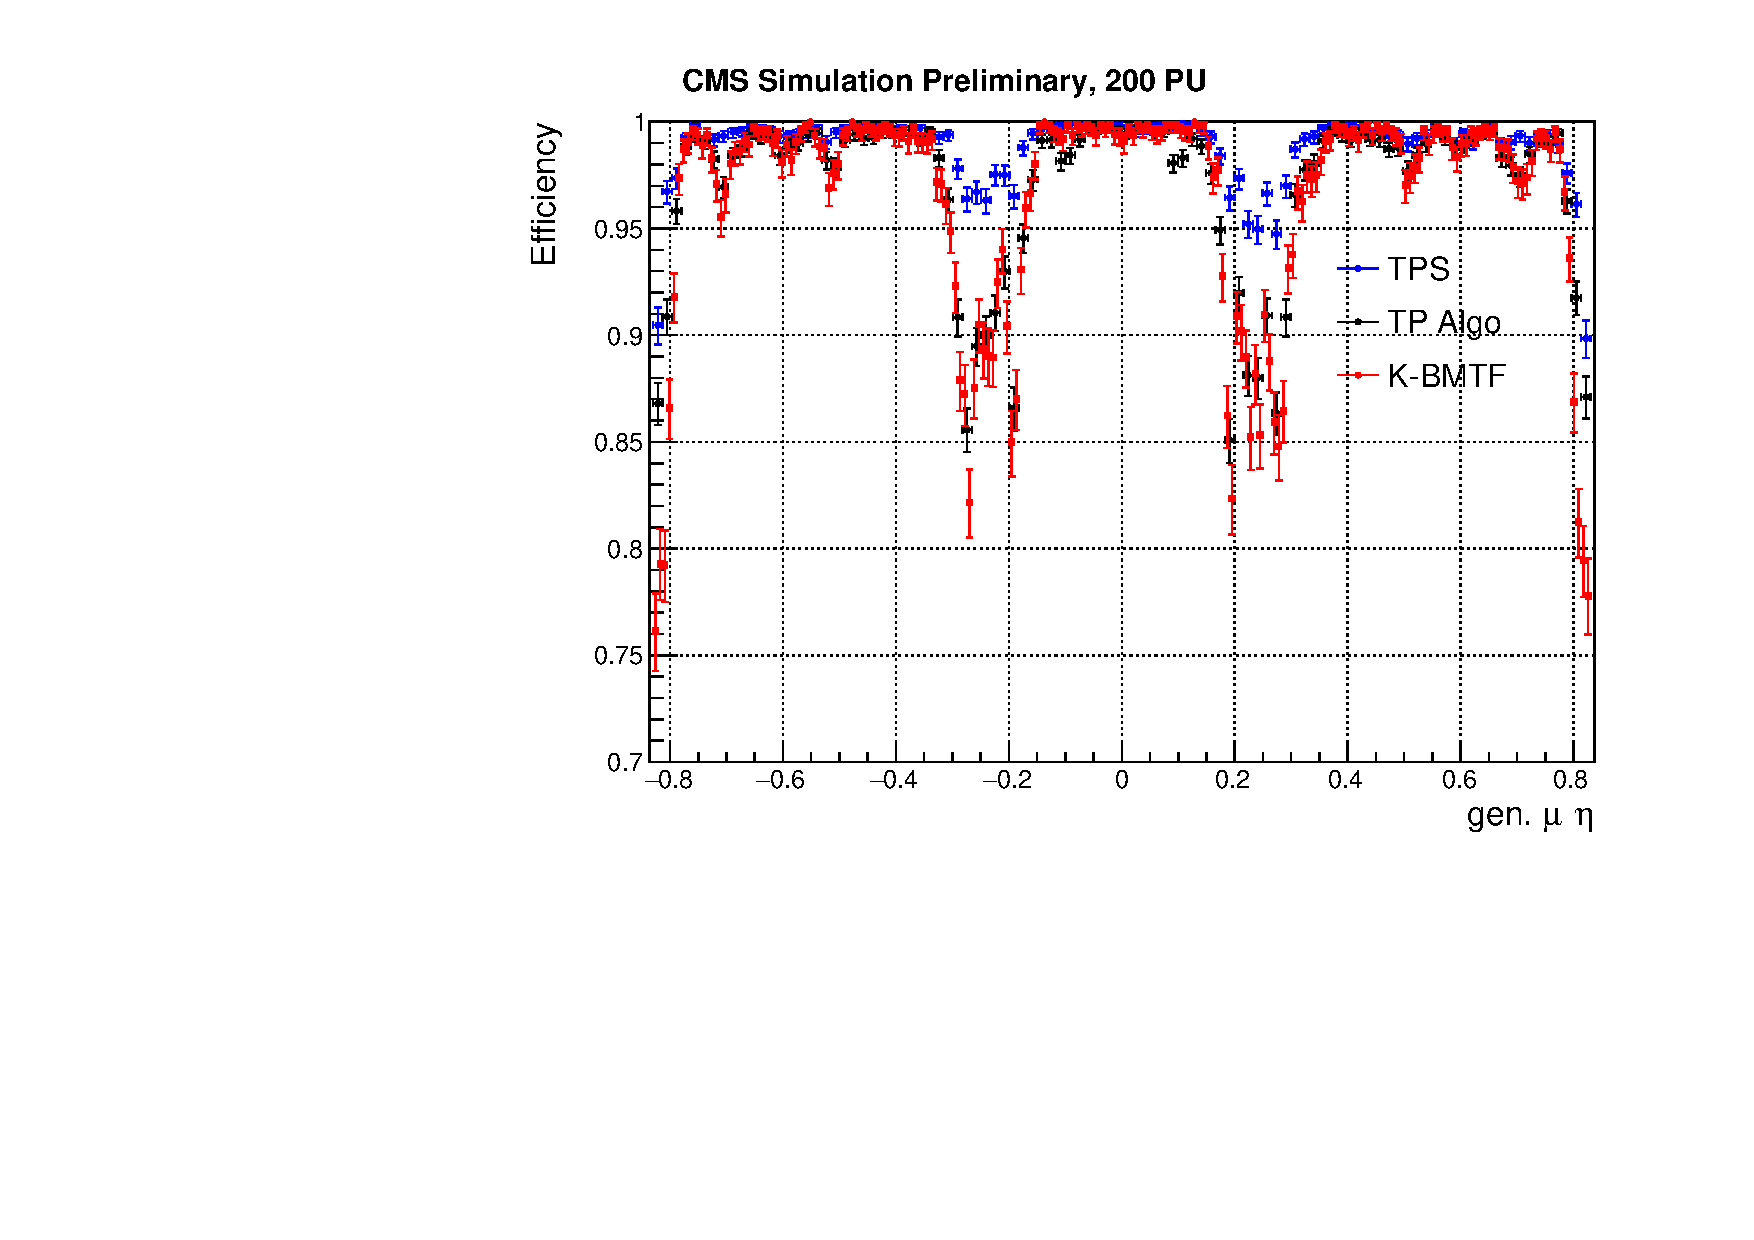
\includegraphics[width=0.48\textwidth]{fig/TPS/effEta20GeV.pdf}
  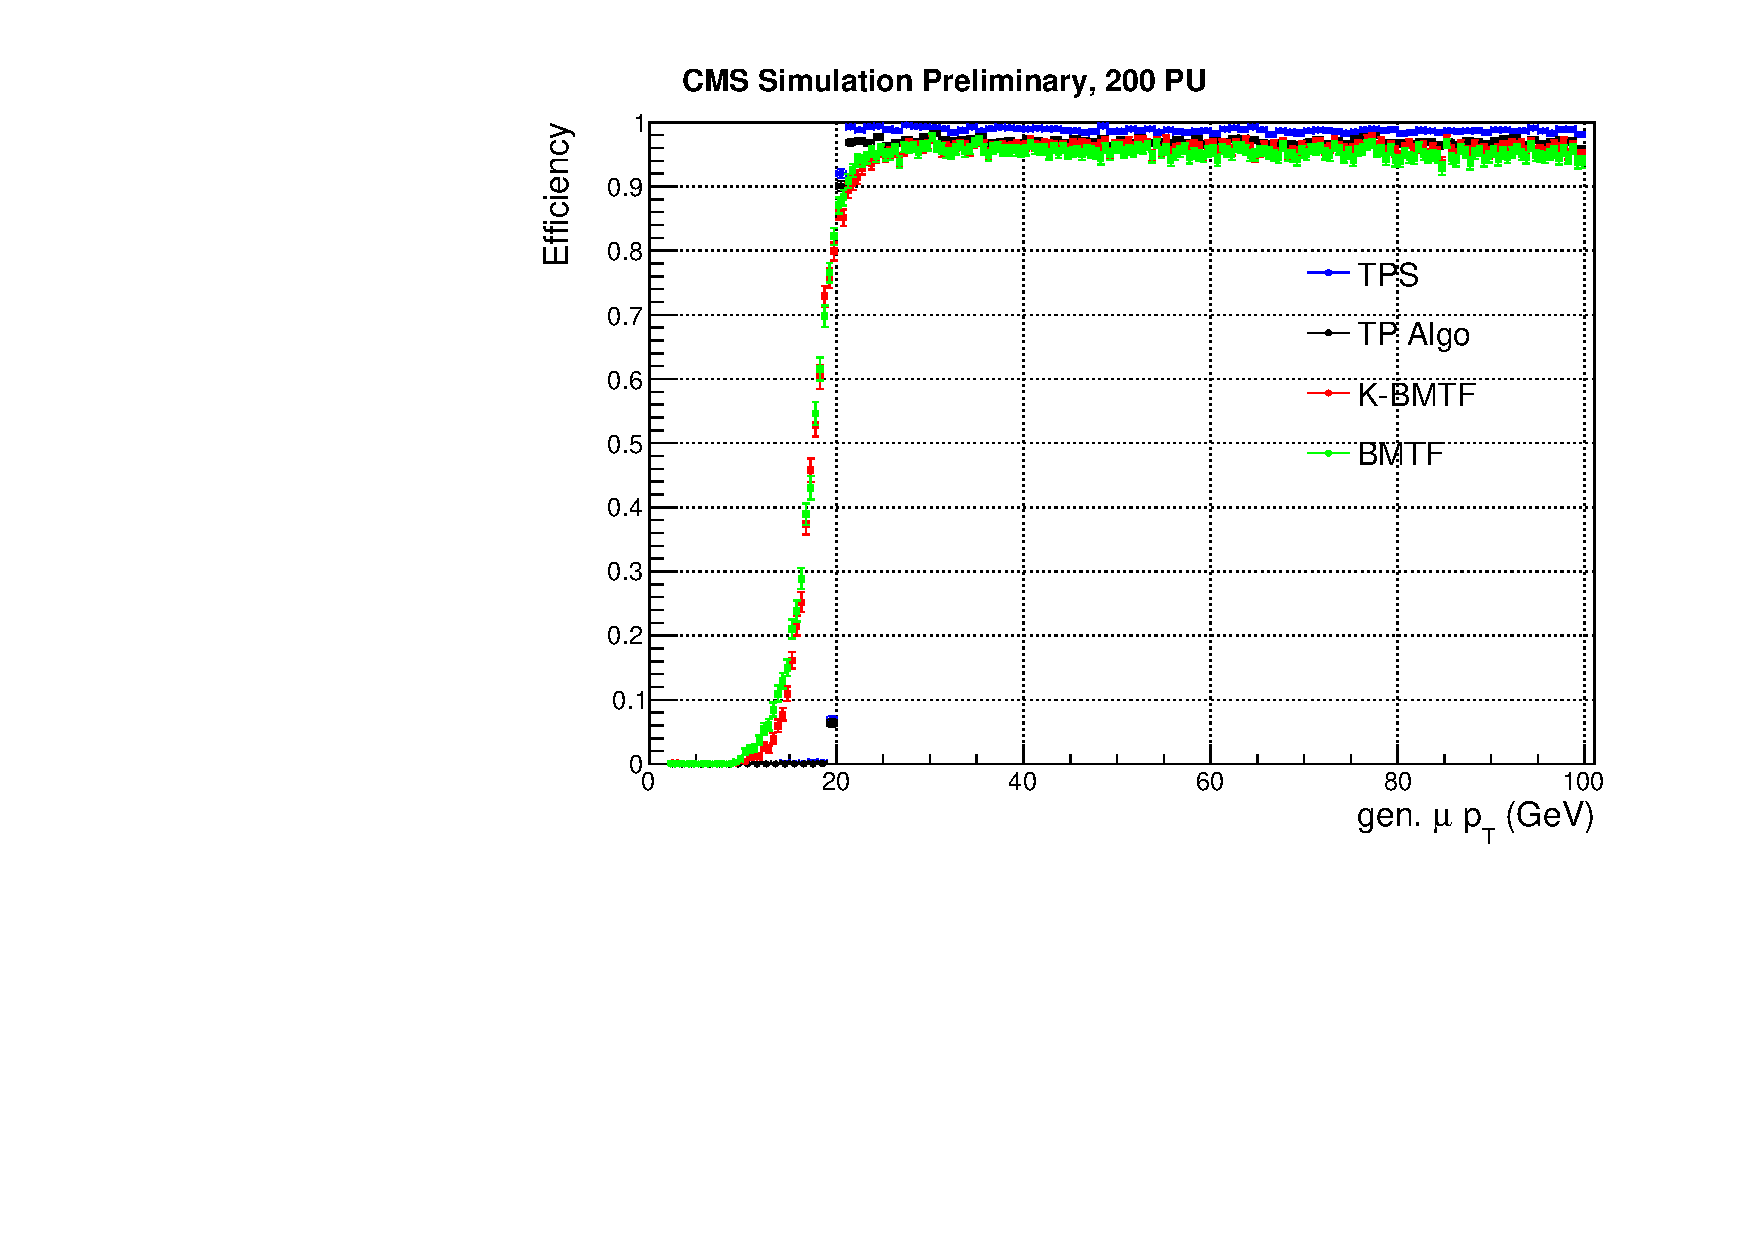
\includegraphics[width=0.48\textwidth]{fig/TPS/effPt20GeV.pdf}
  \caption{Comparison of the efficiencies defined by equation~\ref{eq:eff} for simulated muon $\eta$ (left) and \pt (right). The TPS algorithm is required to have two or more stubs associated to muon tracks, and is compared to the existing BMTF, proposed K-BMTF and TP algorithms. The TPS algorithm offers better overall efficiency in comparison to the other algorithms.}
  \label{fig:eff}
\end{figure}

% The need for higher trigger bandwidth
One of the main upgrades to the L1 Trigger will be the ability to record events at $750\unit{kHz}$.
The bandwidth needed to record events is a precious resource, and as such it is desirable for a muon tracking algorithm to devote as much of it as possible to recording signal events.
This problem is further exacerbated by pileup, as the HL-LHC could see up to 100-200 collision events at a time along the beam line.
To study the effect of pileup on the trigger rate, we used a simulated background-only sample in which there are no muons present to test how often the TPS algorithm will trigger on false tracks.
The trigger rates are computed according to
\begin{equation}\label{eq:rate} % Check equation
  \mathrm{Rate}(\pt)=\frac{f}{N_\mathrm{event}}\sum_{p=\pt}^\infty\mathrm{Max}(p).
\end{equation}

% Trigger rates comparison
A comparison of the trigger rate at different trigger thresholds can be see in figure~\ref{fig:rates}.
The TPS algorithm performance is similar to the TP algo ($\sim8\unit{kHz}$ at $20\unit{GeV}$), and both are significantly lower than the K-BMTF.
Moreover, allowing for track isolation with a maximum $p_{\mathrm{T},cone}$ of $5\unit{GeV}$ and a minimum $p_{\mathrm{T,i}}$ of $2\unit{GeV}$ results in a decrease in the rate by a factor of 2 at $20\unit{GeV}$, thereby demonstrating the effectiveness of using track isolation to suppress background.
These results also show that the TPS algorithm is well-suited for handling background noise while also efficiently matching detection stubs to real muon tracks.

\begin{figure}[htbp] % Need to update figure
  \centering
  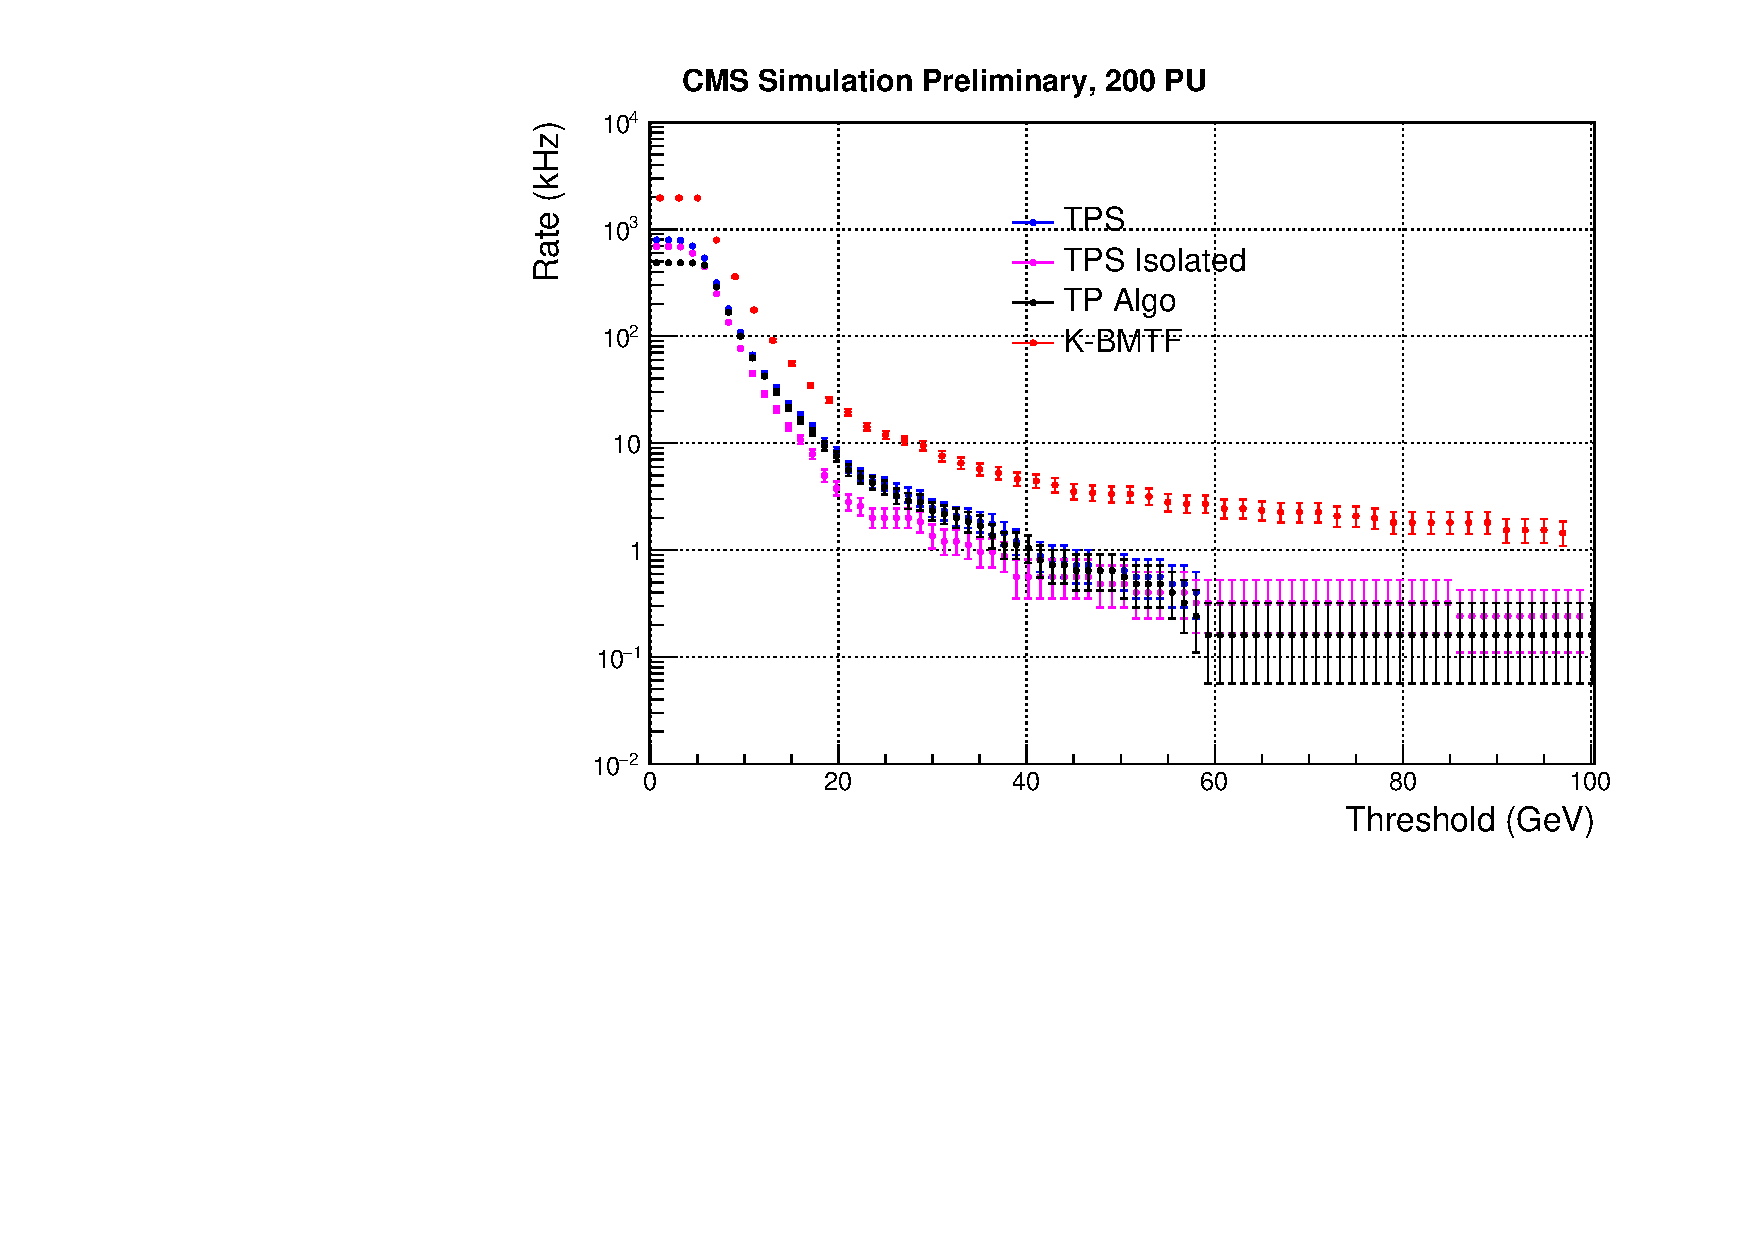
\includegraphics[width=0.48\textwidth]{fig/TPS/rate.pdf}
  \caption{Comparison of the trigger rates at different \pt thresholds for TPS (with and without track isolation), TP, and K-BMTF algorithms when running on a background-only sample in which there are no muons present. Both the TPS and TP algorithms perform better at suppressing fake tracks compared to the K-BMTF over the full \pt threshold range.}
  \label{fig:rates}
\end{figure}

\section{Future Implementation}
\label{subsec:TPSResults}

% Implementation on the OCEAN board
While initially tested as software, the TPS algorithm will eventually be implemented into the CMS detector through hardware to allow for fast processing.
As of this writing, the UCLA CMS research group is currently in the process of designing and testing a custom OCEAN Blade board with an FPGA that will allow for the TPS algorithm to be implemented as firmware.
% More up-to-date information on resource usage and performance results here

\begin{figure}[htbp] % Need to update figure
  \centering
  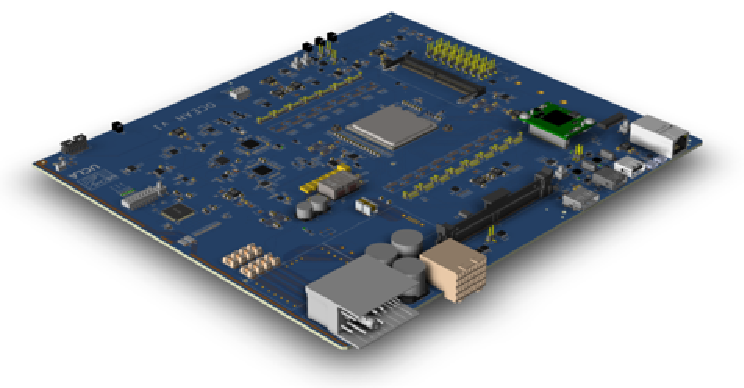
\includegraphics[width=0.48\textwidth]{fig/TPS/ocean.pdf}
  \caption{Render of the OCEAN Blade board that will be implemented into the CMS detector hardware. The onboard FPGA will allow for the TPS algorithm to be implemented directly as firmware into the muon trigger in the detector.}
  \label{fig:ocean}
\end{figure}
